\documentclass{article}
\usepackage[utf8]{inputenc}
\usepackage[T1]{fontenc}
\usepackage[polish]{babel}
\usepackage{float}
\usepackage{amsmath}
\usepackage{graphicx}
\usepackage{amsfonts}
\usepackage{amssymb}
\graphicspath{ {./images/} }

\begin{document}

\title{Analiza Klasyfikacji Posiadaczy Kart Kredytowych}
\author{Karol Kot}
\date{\today}
\maketitle

\section{Opis Zadania}
Pracowano z zestawem danych pochodzącym z banku w Tajwanie, zawierającym informacje o posiadaczach kart kredytowych i ich zwyczajach wydatkowych.
Zbiór danych zawiera ponad 30,000 obserwacji, z klientami sklasyfikowanymi jako wiarygodni (credible) lub ryzykowni (uncredible), gdzie ci drudzy stanowią 20\% zbioru danych.
Celem było przetestowanie i porównanie wyników klasyfikatorów na danych oryginalnych, oversamplowanych, undersamplowanych oraz z SMOTE,
oraz ocena wpływu selekcji cech na skuteczność klasyfikacji.

\section{Analiza danych}
\subsection{Wykres korelacji}
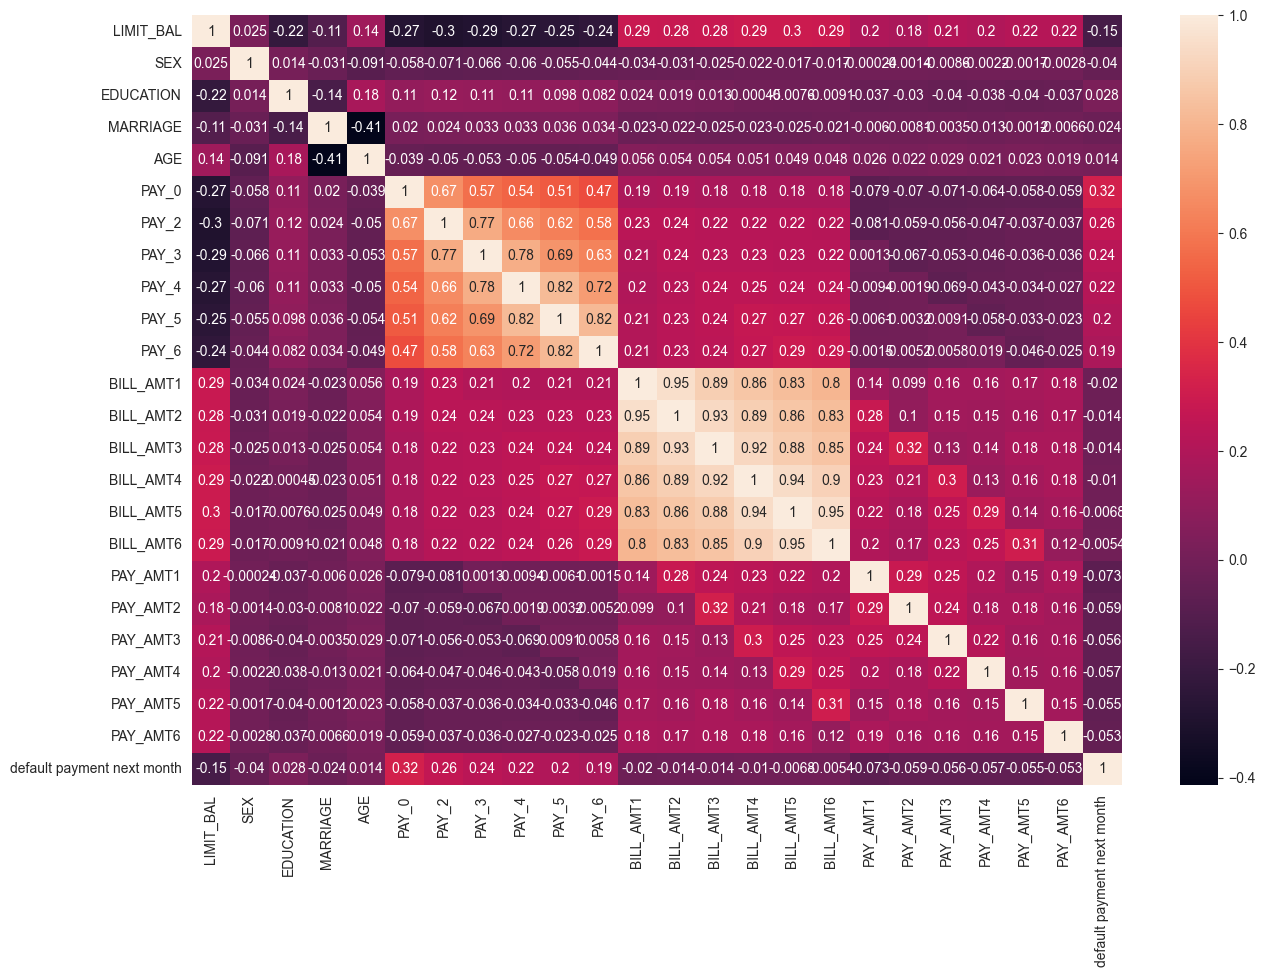
\includegraphics[width=1\textwidth]{./corelation.png}

\subsection{Srednie wartości atrybutów i standardowe odchylenia atrybutów}
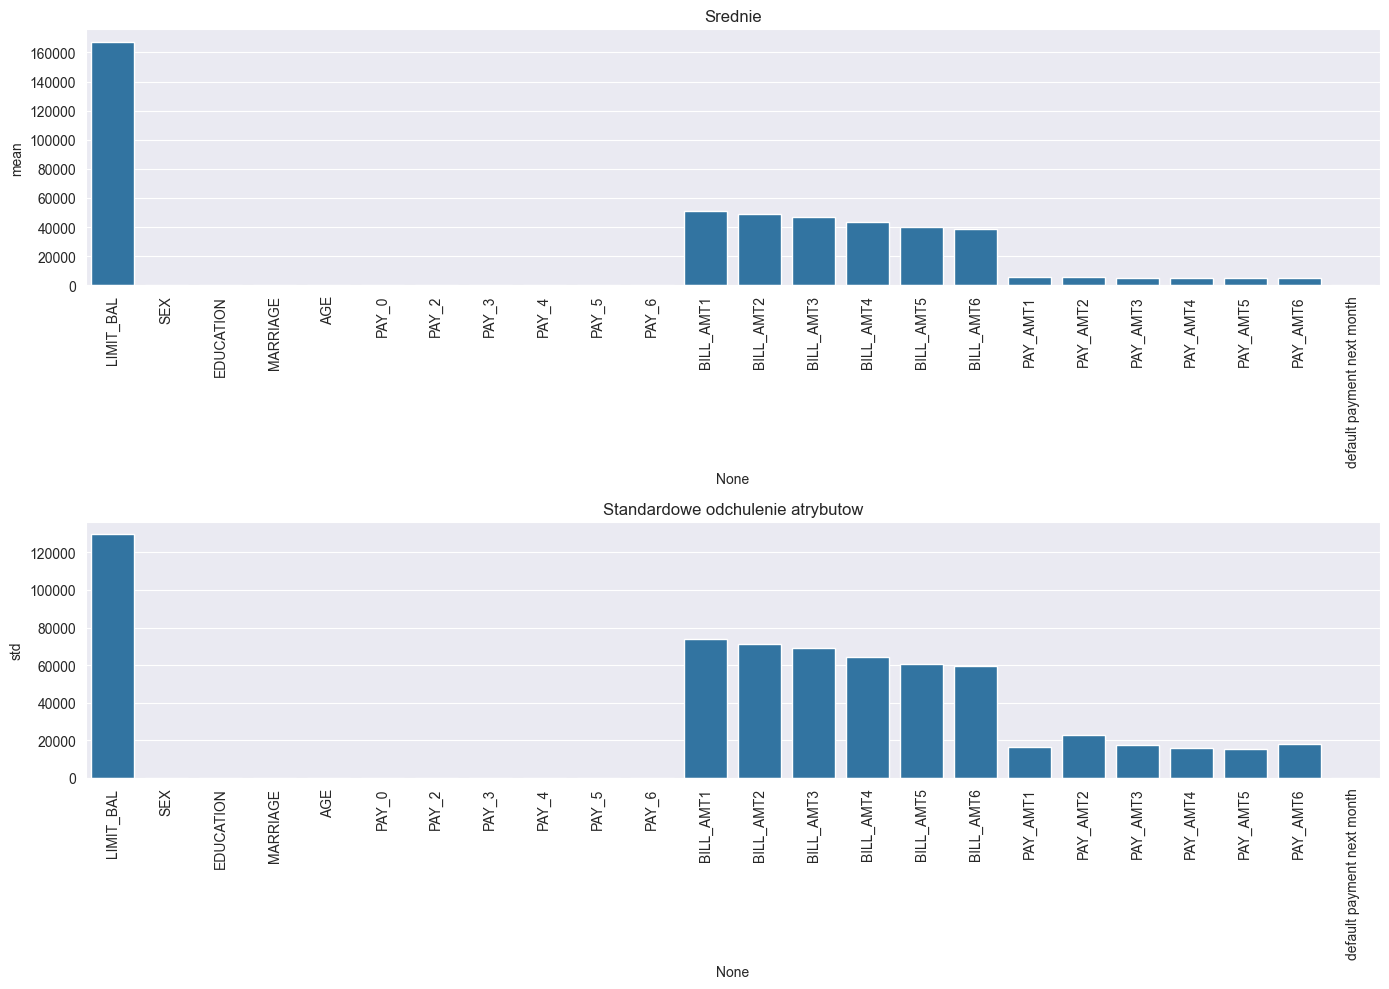
\includegraphics[width=1\textwidth]{./srednie.png}

\subsection{Wykresy pudełkowe}
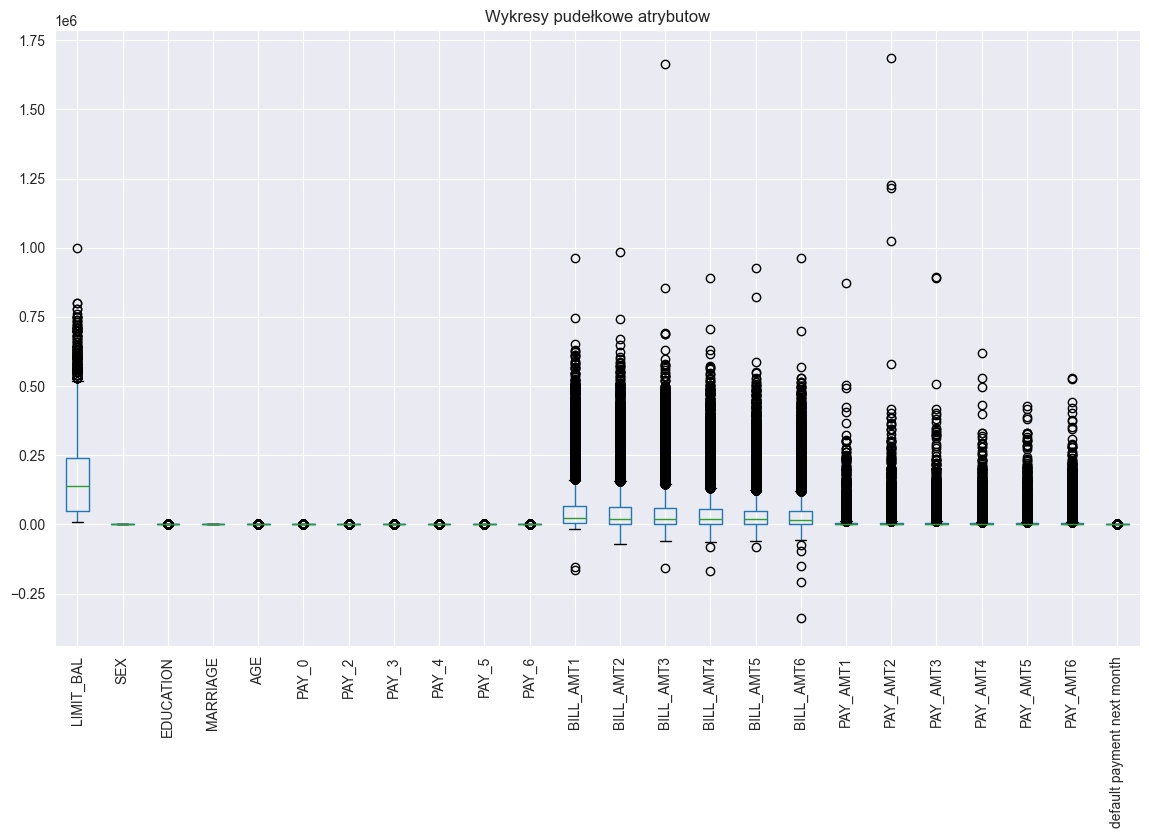
\includegraphics[width=1\textwidth]{./box_plots.png}

\subsection{Histogramy}
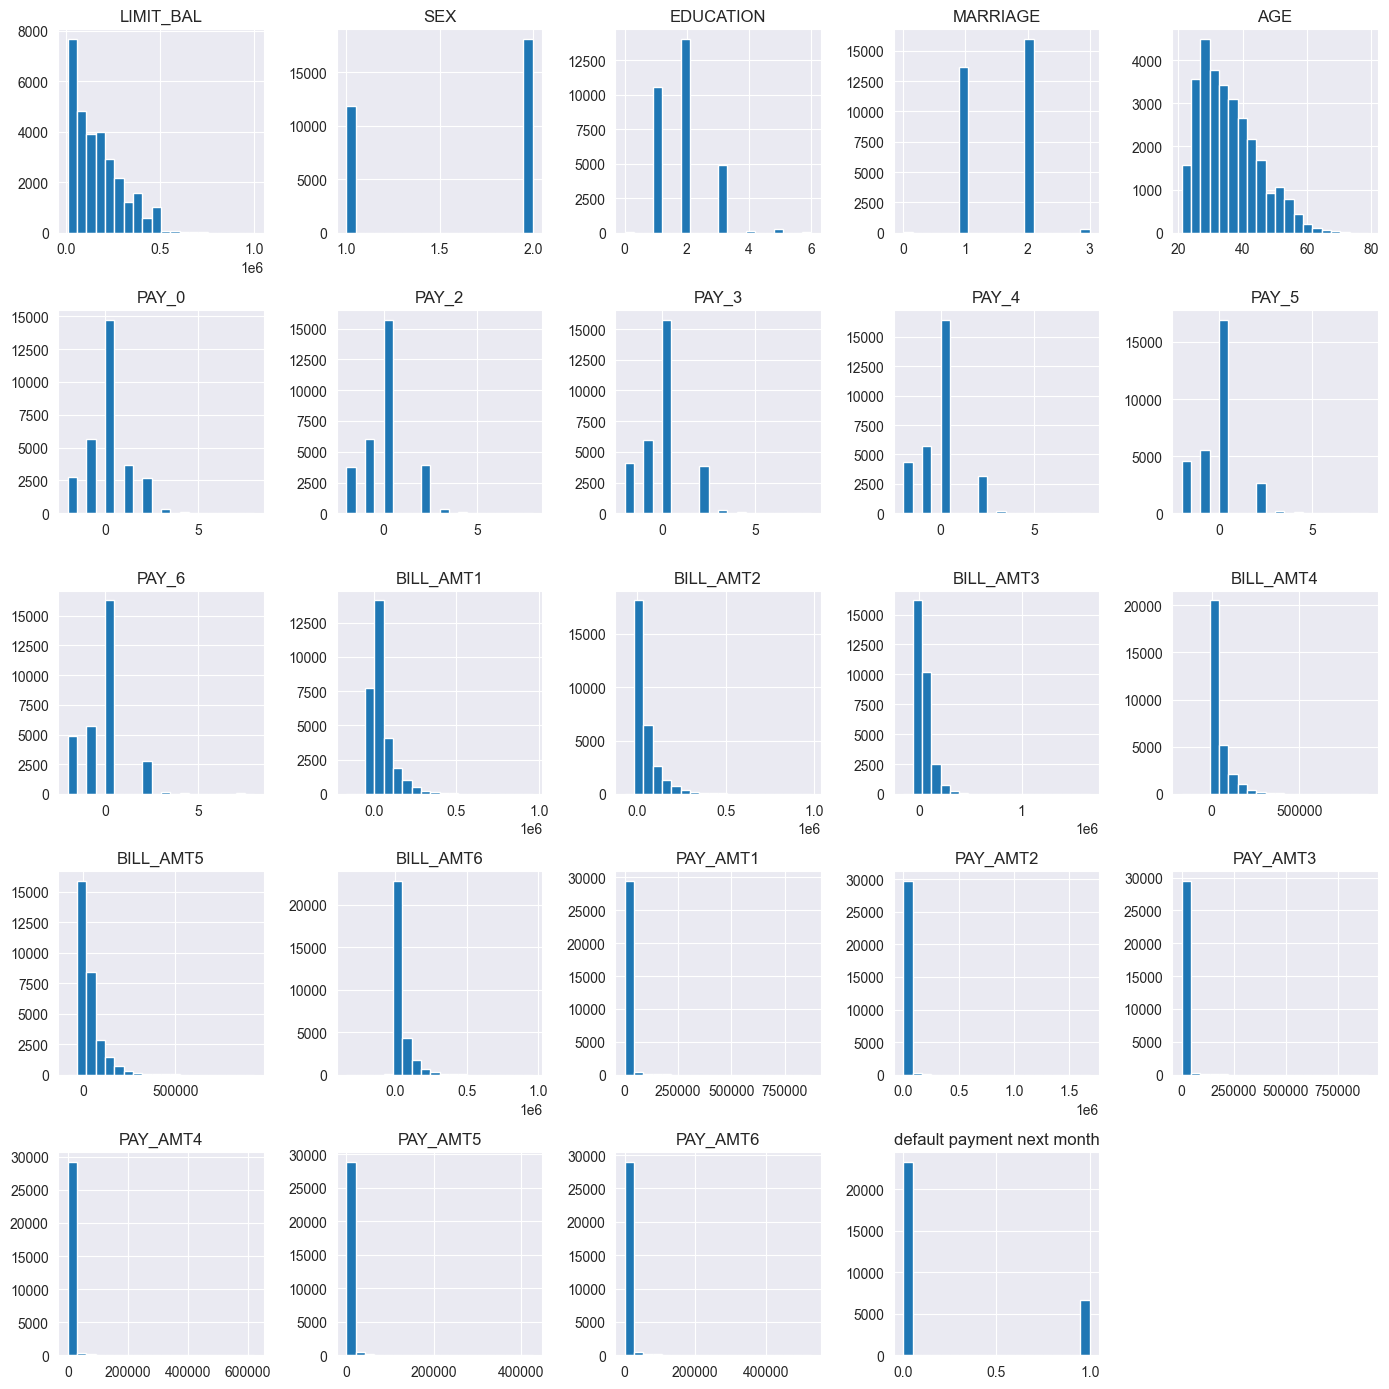
\includegraphics[width=1\textwidth]{./histogramy.png}

\section{Odpowiedzi na Pytania}

\subsection{Testowanie klasyfikatora na danych oryginalnych}

Wyniki klasyfikatorów na danych oryginalnych:

\begin{itemize}
    \item \textbf{Regresja Logistyczna}:
    \begin{itemize}
        \item Dokładność: 0.8086
        \item AUC: 0.7149
    \end{itemize}
    \item \textbf{XGBoost}:
    \begin{itemize}
        \item Dokładność: 0.8098
        \item AUC: 0.7578
    \end{itemize}
\end{itemize}

Wyniki pokazują, że XGBoost ma nieco wyższą dokładność i znacznie wyższe AUC w porównaniu do regresji logistycznej na danych oryginalnych.

\subsection{Testowanie klasyfikatora na danych oversamplowanych, undersamplowanych i z SMOTE}

Wyniki klasyfikatorów na różnych metodach próbkowania:

\begin{itemize}
    \item \textbf{Dane oversamplowane}:
    \begin{itemize}
        \item Regresja Logistyczna:
        \begin{itemize}
            \item Dokładność: 0.6836
            \item AUC: 0.7155
        \end{itemize}
        \item XGBoost:
        \begin{itemize}
            \item Dokładność: 0.7606
            \item AUC: 0.7570
        \end{itemize}
    \end{itemize}
    \item \textbf{Dane undersamplowane}:
    \begin{itemize}
        \item Regresja Logistyczna:
        \begin{itemize}
            \item Dokładność: 0.6807
            \item AUC: 0.7166
        \end{itemize}
        \item XGBoost:
        \begin{itemize}
            \item Dokładność: 0.7053
            \item AUC: 0.7522
        \end{itemize}
    \end{itemize}
    \item \textbf{Dane z SMOTE}:
    \begin{itemize}
        \item Regresja Logistyczna:
        \begin{itemize}
            \item Dokładność: 0.6713
            \item AUC: 0.7176
        \end{itemize}
        \item XGBoost:
        \begin{itemize}
            \item Dokładność: 0.8058
            \item AUC: 0.7557
        \end{itemize}
    \end{itemize}
\end{itemize}

Wyniki wskazują, że XGBoost konsekwentnie osiąga lepsze wyniki zarówno pod względem dokładności, jak i AUC we wszystkich metodach próbkowania w porównaniu do regresji logistycznej. Oversampling i SMOTE przynoszą większe korzyści dla modelu XGBoost niż undersampling.

\subsection{Porównanie wyników oraz obserwacje i wnioski}

\subsubsection{Obserwacje}
\begin{itemize}
    \item \textbf{Wydajność na danych oryginalnych}: XGBoost przewyższa regresję logistyczną pod względem AUC, co wskazuje na lepszą separację klas.
    \item \textbf{Wpływ metod próbkowania}:
    \begin{itemize}
        \item \textbf{Oversampling}: Poprawia AUC dla XGBoost, ale nie tak bardzo dla regresji logistycznej.
        \item \textbf{Undersampling}: Powoduje niższą dokładność dla obu modeli, ale AUC pozostaje stosunkowo stabilne.
        \item \textbf{SMOTE}: Zapewnia zrównoważoną poprawę AUC dla obu modeli, przy czym XGBoost znacząco zyskuje na dokładności.
    \end{itemize}
\end{itemize}

\subsubsection{Wnioski}
\begin{itemize}
    \item \textbf{Wybór modelu}: XGBoost jest ogólnie bardziej efektywny niż regresja logistyczna dla tego zbioru danych, szczególnie pod względem AUC.
    \item \textbf{Metody próbkowania}: SMOTE i oversampling są bardziej efektywne niż undersampling w poprawie wydajności modeli, szczególnie dla XGBoost.
    \item \textbf{AUC jako metryka}: AUC jest kluczową metryką w tym niezbalansowanym zbiorze danych, ponieważ lepiej odzwierciedla zdolność modelu do rozróżniania między klasami wiarygodnymi i niewiarygodnymi niż sama dokładność.
\end{itemize}

\subsection{Czy selekcja cech zwiększa skuteczność klasyfikacji?}

\subsubsection{Wyniki selekcji cech}

\begin{itemize}
    \item \textbf{Wybrane cechy przy użyciu RFE}:
    \begin{itemize}
        \item Regresja Logistyczna:
        \begin{itemize}
            \item Dokładność: 0.8087
            \item AUC: 0.6975
        \end{itemize}
        \item XGBoost:
        \begin{itemize}
            \item Dokładność: 0.8140
            \item AUC: 0.7389
        \end{itemize}
    \end{itemize}
    \item \textbf{Wybrane cechy przy użyciu SFS}:
    \begin{itemize}
        \item Regresja Logistyczna:
        \begin{itemize}
            \item Dokładność: 0.8118
            \item AUC: 0.7062
        \end{itemize}
        \item XGBoost:
        \begin{itemize}
            \item Dokładność: 0.8128
            \item AUC: 0.7429
        \end{itemize}
    \end{itemize}
\end{itemize}

\subsection{Wybór cech przy użyciu SFS i RFE}
\textbf{Wybrane cechy przy użyciu RFE}:
\begin{itemize}
    \item SEX
    \item EDUCATION
    \item MARRIAGE
    \item AGE
    \item PAY\_0
    \item PAY\_2
    \item PAY\_3
    \item PAY\_4
    \item PAY\_5
    \item PAY\_6
\end{itemize}

\textbf{Wybrane cechy przy użyciu SFS}:
\begin{itemize}
    \item SEX
    \item EDUCATION
    \item MARRIAGE
    \item AGE
    \item PAY\_0
    \item PAY\_AMT1
    \item PAY\_AMT2
    \item PAY\_AMT3
    \item PAY\_AMT4
    \item PAY\_AMT5
\end{itemize}

\subsubsection{Wykresy ważności cech}

W celu oceny ważności cech dla regresji logistycznej oraz XGBoost, zastosowano następujące funkcje - metody zostaly uzyte obok RFE i SFS:

\begin{verbatim}
def plot_lr_feature_importance(model, feature_names):
    importance = np.abs(model.coef_[0])
    feature_importance = pd.Series(importance, index=feature_names).sort_values(ascending=False)
    feature_importance.plot(kind='bar', figsize=(12, 8))
    plt.title('Logistic Regression Feature Importance')
    plt.ylabel('Importance')
    plt.show()
    return feature_importance

def plot_xgb_feature_importance(model, feature_names):
    plt.figure(figsize=(12, 8))
    plot_importance(model, max_num_features=20, importance_type='weight')
    plt.title('XGBoost Feature Importance')
    plt.show()
    importance = model.get_booster().get_score(importance_type='weight')
    importance_mapped = {feature_names[int(k[1:])]: v for k, v in importance.items()}
    return importance_mapped
\end{verbatim}

\textbf{Wyniki regresji logistycznej}:
\begin{figure}[H]
    \centering
    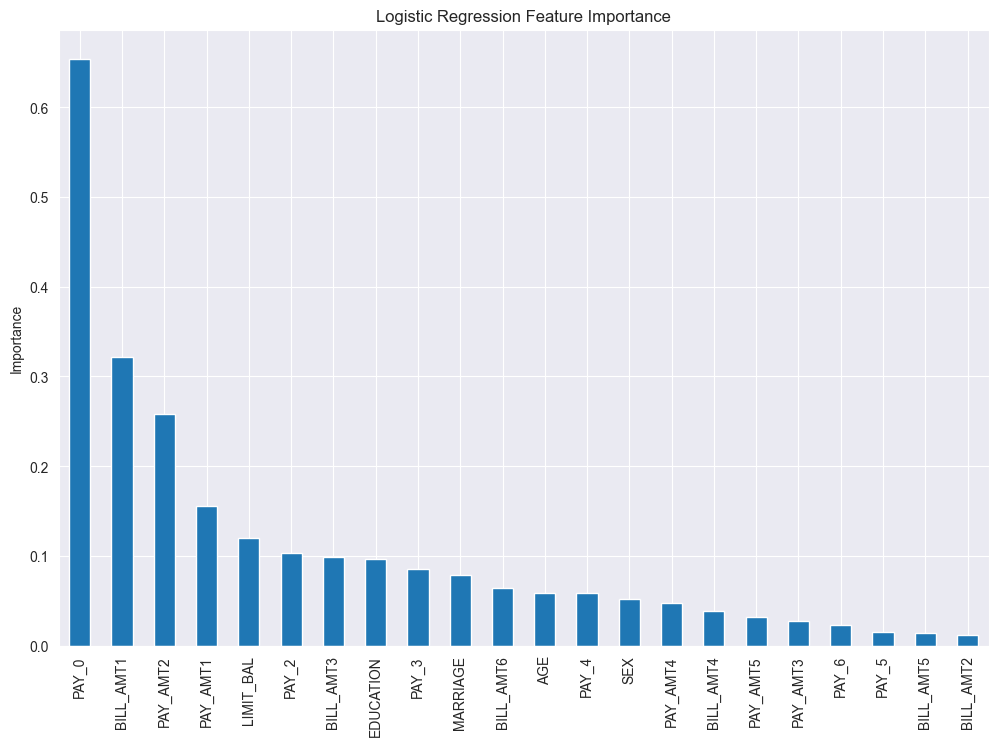
\includegraphics[width=0.8\textwidth]{./lr_importance.png}
    \caption{Wykres ważności cech - Regresja Logistyczna}
    \label{fig:lr_feature_importance}
\end{figure}

\textbf{Wyniki XGBoost}:
\begin{figure}[H]
    \centering
    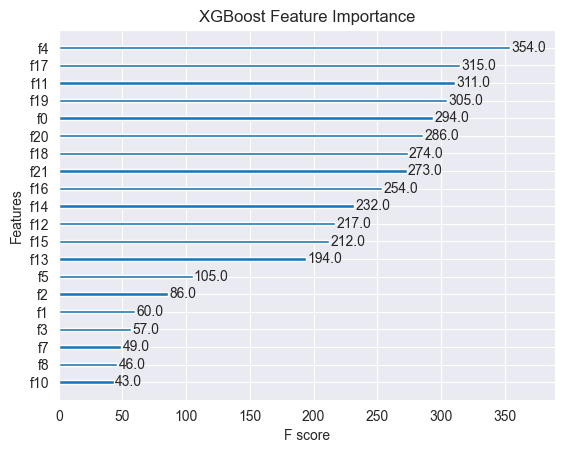
\includegraphics[width=0.8\textwidth]{./xgb_importance.png}
    \caption{Wykres ważności cech - XGBoost}
    \label{fig:xgb_feature_importance}
\end{figure}


\subsubsection{Obserwacje}
\begin{itemize}
    \item \textbf{Regresja Logistyczna}: Selekcja cech nieznacznie poprawia dokładność, ale ma mieszany wpływ na AUC.
    \item \textbf{XGBoost}: Selekcja cech znacząco poprawia zarówno dokładność, jak i AUC, przy czym SFS daje nieco lepsze wyniki niż RFE.
\end{itemize}

\subsubsection{Wnioski}
\begin{itemize}
    \item \textbf{Efektywność selekcji cech}: Selekcja cech, szczególnie przy użyciu SFS, poprawia wydajność klasyfikacji dla XGBoost. W przypadku regresji logistycznej wpływ jest mniej wyraźny, ale nadal korzystny pod względem dokładności.
    \item \textbf{Rekomendacja}: Stosowanie metod selekcji cech, takich jak RFE i SFS, może znacząco poprawić wydajność modelu, zwłaszcza w przypadku bardziej złożonych modeli jak XGBoost.
\end{itemize}


\end{document}